\documentclass[11pt]{article}
\makeatletter\if@twocolumn\PassOptionsToPackage{switch}{lineno}\else\fi\makeatother

      \makeatletter
\usepackage{wrapfig}
\newcounter{aubio}

\long\def\bioItem{%
\@ifnextchar[{\@bioItem}{\@@bioItem}}

\long\def\@bioItem[#1]#2#3{
 \stepcounter{aubio}
 \expandafter\gdef\csname authorImage\theaubio\endcsname{#1}
 \expandafter\gdef\csname authorName\theaubio\endcsname{#2}
 \expandafter\gdef\csname authorDetails\theaubio\endcsname{#3}
}

\long\def\@@bioItem#1#2{
 \stepcounter{aubio}
 \expandafter\gdef\csname authorName\theaubio\endcsname{#1}
 \expandafter\gdef\csname authorDetails\theaubio\endcsname{#2}
}

\newcommand{\checkheight}[1]{%
  \par \penalty-100\begingroup%
  \setbox8=\hbox{#1}%
  \setlength{\dimen@}{\ht8}%
  \dimen@ii\pagegoal \advance\dimen@ii-\pagetotal
  \ifdim \dimen@>\dimen@ii
    \break
  \fi\endgroup}

\def\printBio{%
  \@tempcnta=0
   \loop
     \advance \@tempcnta by 1
     \def\aubioCnt{\the\@tempcnta}
     \setlength{\intextsep}{0pt}%
     \setlength{\columnsep}{10pt}%
     \newbox\boxa%
     \setbox\boxa\vbox{\csname authorDetails\aubioCnt\endcsname}
     \expandafter\ifx\csname authorImage\aubioCnt\endcsname\relax%
      \else%
       \checkheight{\includegraphics[height=1.25in,width=1in,keepaspectratio]{\csname authorImage\aubioCnt\endcsname}}
        \begin{wrapfigure}{l}{25mm}
         \includegraphics[height=1.25in,width=1in,keepaspectratio]{\csname authorImage\aubioCnt\endcsname}%height=145pt
        \end{wrapfigure}\par
      \fi
     {\parindent0pt\textbf{\csname authorName\aubioCnt\endcsname}\csname authorDetails\aubioCnt\endcsname \par\bigskip%
     \expandafter\ifx\csname authorImage\aubioCnt\endcsname\relax\else%
      \ifdim\the\ht\boxa < 90pt\vskip\dimexpr(90pt -\the\ht\boxa-1pc)\fi%
     \fi}%for adding additional vskip for avoiding image overlap.
      \ifnum\@tempcnta < \theaubio
   \repeat
   }

\makeatother

      



\usepackage{amsfonts,amssymb,amsbsy,latexsym,amsmath,tabulary,graphicx,times,xcolor}
\usepackage[utf8x]{inputenc}
\usepackage{fancyhdr}
\def\NormalBaseline{\def\baselinestretch{1.1}}
\makeatletter
\def\hlinewd#1{%
  \noalign{\ifnum0=`}\fi\hrule \@height #1%
  \futurelet\reserved@a\@xhline}
\def\tbltoprule{\hlinewd{.8pt}}%\\[-10pt]}
\def\tblbottomrule{\hlinewd{.8pt}}
\def\tblmidrule{\hline\noalign{\vspace*{2pt}}}

\def\@shorttitle{\@empty}
\def\shorttitle#1{\gdef\@shorttitle{#1}}

\fancypagestyle{custom}{
\fancyhf{}
\fancyhead[C]{\@shorttitle}
\fancyhead[R]{\thepage}
\fancyfoot[C]{}
\renewcommand\headrulewidth{0.4pt}
\renewcommand\footrulewidth{0pt}
}
\fancypagestyle{plain}{
\fancyhf{}
\renewcommand\headrulewidth{0.4pt}
}


\makeatother

\usepackage{times}

\usepackage[a4paper,margin=2.5cm,headsep=.7cm,headheight=18pt,top=3cm,footnotesep=1.5\baselineskip]{geometry}
\usepackage{caption}
\captionsetup[figure]{labelfont=bf,labelsep=newline,justification=centerlast,labelfont={small,sc,bf},font=small,aboveskip=.3\baselineskip}

\captionsetup[table]{labelfont=bf,labelsep=newline,justification=centerlast,labelfont={small,sc,bf},font=small,aboveskip=.3\baselineskip}
\linespread{1.5}

\setcounter{totalnumber}{4}
\def\topfraction{0.9}
\def\bottomfraction{0.4}
\def\floatpagefraction{0.8}
\def\textfraction{0.1}
\widowpenalty 10000
\clubpenalty 10000
\makeatletter
\setlength\intextsep   {1.5\baselineskip \@plus 2\p@ \@minus 2\p@}
\makeatother

  
%%%%%%%%%%%%%%%%%%%%%%%%%%%%%%%%%%%%%%%%%%%%%%%%%%%%%%%%%%%%%%%%%%%%%%%%%%
% Following additional macros are required to function some 
% functions which are not available in the class used.
%%%%%%%%%%%%%%%%%%%%%%%%%%%%%%%%%%%%%%%%%%%%%%%%%%%%%%%%%%%%%%%%%%%%%%%%%%
\usepackage{url,multirow,morefloats,floatflt,cancel,tfrupee}
\makeatletter


\AtBeginDocument{\@ifpackageloaded{textcomp}{}{\usepackage{textcomp}}}
\makeatother
\usepackage{colortbl}
\usepackage{xcolor}
\usepackage{pifont}
\usepackage[nointegrals]{wasysym}
\urlstyle{rm}
\makeatletter

%%%For Table column width calculation.
\def\mcWidth#1{\csname TY@F#1\endcsname+\tabcolsep}

%%Hacking center and right align for table
\def\cAlignHack{\rightskip\@flushglue\leftskip\@flushglue\parindent\z@\parfillskip\z@skip}
\def\rAlignHack{\rightskip\z@skip\leftskip\@flushglue \parindent\z@\parfillskip\z@skip}

%Etal definition in references
\@ifundefined{etal}{\def\etal{\textit{et~al}}}{}


%\if@twocolumn\usepackage{dblfloatfix}\fi
\usepackage{ifxetex}
\ifxetex\else\if@twocolumn\@ifpackageloaded{stfloats}{}{\usepackage{dblfloatfix}}\fi\fi

\AtBeginDocument{
\expandafter\ifx\csname eqalign\endcsname\relax
\def\eqalign#1{\null\vcenter{\def\\{\cr}\openup\jot\m@th
  \ialign{\strut$\displaystyle{##}$\hfil&$\displaystyle{{}##}$\hfil
      \crcr#1\crcr}}\,}
\fi
}

%For fixing hardfail when unicode letters appear inside table with endfloat
\AtBeginDocument{%
  \@ifpackageloaded{endfloat}%
   {\renewcommand\efloat@iwrite[1]{\immediate\expandafter\protected@write\csname efloat@post#1\endcsname{}}}{\newif\ifefloat@tables}%
}%

\def\BreakURLText#1{\@tfor\brk@tempa:=#1\do{\brk@tempa\hskip0pt}}
\let\lt=<
\let\gt=>
\def\processVert{\ifmmode|\else\textbar\fi}
\let\processvert\processVert

\@ifundefined{subparagraph}{
\def\subparagraph{\@startsection{paragraph}{5}{2\parindent}{0ex plus 0.1ex minus 0.1ex}%
{0ex}{\normalfont\small\itshape}}%
}{}

% These are now gobbled, so won't appear in the PDF.
\newcommand\role[1]{\unskip}
\newcommand\aucollab[1]{\unskip}
  
\@ifundefined{tsGraphicsScaleX}{\gdef\tsGraphicsScaleX{1}}{}
\@ifundefined{tsGraphicsScaleY}{\gdef\tsGraphicsScaleY{.9}}{}
% To automatically resize figures to fit inside the text area
\def\checkGraphicsWidth{\ifdim\Gin@nat@width>\linewidth
	\tsGraphicsScaleX\linewidth\else\Gin@nat@width\fi}

\def\checkGraphicsHeight{\ifdim\Gin@nat@height>.9\textheight
	\tsGraphicsScaleY\textheight\else\Gin@nat@height\fi}

\def\fixFloatSize#1{}%\@ifundefined{processdelayedfloats}{\setbox0=\hbox{\includegraphics{#1}}\ifnum\wd0<\columnwidth\relax\renewenvironment{figure*}{\begin{figure}}{\end{figure}}\fi}{}}
\let\ts@includegraphics\includegraphics

\def\inlinegraphic[#1]#2{{\edef\@tempa{#1}\edef\baseline@shift{\ifx\@tempa\@empty0\else#1\fi}\edef\tempZ{\the\numexpr(\numexpr(\baseline@shift*\f@size/100))}\protect\raisebox{\tempZ pt}{\ts@includegraphics{#2}}}}

%\renewcommand{\includegraphics}[1]{\ts@includegraphics[width=\checkGraphicsWidth]{#1}}
\AtBeginDocument{\def\includegraphics{\@ifnextchar[{\ts@includegraphics}{\ts@includegraphics[width=\checkGraphicsWidth,height=\checkGraphicsHeight,keepaspectratio]}}}

\DeclareMathAlphabet{\mathpzc}{OT1}{pzc}{m}{it}

\def\URL#1#2{\@ifundefined{href}{#2}{\href{#1}{#2}}}

%%For url break
\def\UrlOrds{\do\*\do\-\do\~\do\'\do\"\do\-}%
\g@addto@macro{\UrlBreaks}{\UrlOrds}



\edef\fntEncoding{\f@encoding}
\def\EUoneEnc{EU1}
\makeatother
\def\floatpagefraction{0.8} 
\def\dblfloatpagefraction{0.8}
\def\style#1#2{#2}
\def\xxxguillemotleft{\fontencoding{T1}\selectfont\guillemotleft}
\def\xxxguillemotright{\fontencoding{T1}\selectfont\guillemotright}

\newif\ifmultipleabstract\multipleabstractfalse%
\newenvironment{typesetAbstractGroup}{}{}%

%%%%%%%%%%%%%%%%%%%%%%%%%%%%%%%%%%%%%%%%%%%%%%%%%%%%%%%%%%%%%%%%%%%%%%%%%%

\usepackage{natbib}




\usepackage{titlesec}
\usepackage[T1]{fontenc}
\setcounter{secnumdepth}{5}
 
\titleformat{\section}[hang]{\NormalBaseline\filright\large\bfseries}
{\large\thesection}
{10pt}
{}
[]
\titleformat{\subsection}[hang]{\NormalBaseline\filright\bfseries}
{\thesubsection}
{10pt}
{}
[]
\titleformat{\subsubsection}[hang]{\NormalBaseline\filright\bfseries\itshape}
{\upshape\thesubsubsection}
{10pt}
{}
[]
\titleformat{\paragraph}[runin]{\NormalBaseline\filright\bfseries}
{\theparagraph}
{10pt}
{}
[]
\titleformat{\subparagraph}[runin]{\NormalBaseline\filright\bfseries\itshape}
{\thesubparagraph}
{10pt}
{}
[]

\titlespacing{\section}{0pt}{1.5\baselineskip}{.2\baselineskip}  
\titlespacing{\subsection}{0pt}{1.5\baselineskip}{.2\baselineskip}  
\titlespacing{\subsubsection}{0pt}{1.5\baselineskip}{.2\baselineskip}  
\titlespacing{\paragraph}{0pt}{.5\baselineskip}{10pt}  
\titlespacing{\subparagraph}{0pt}{.5\baselineskip}{10pt}  
  

  




\usepackage{float}

\begin{document}



\renewcommand*\rmdefault{bch}\normalfont\upshape

\shorttitle{Class Assignment}

\date{}  

  
\title{\NormalBaseline\raggedright\bfseries Multiple Sequence Alignment of SARS-CoV-2 genes}
  \let\origthanks\thanks
\renewcommand\thanks[1]{\begingroup\let\rlap\relax\origthanks{#1}\endgroup}
\author{\hskip2pc\parbox{.95\textwidth}{\bfseries\large Antonio Osamu Katagiri Tanaka\textsuperscript{1}\thanks{E-mail: A01212611@itesm.mx}
      \\[3pt] 
    % Address
    \normalfont\itshape\NormalBaseline \textsuperscript{\upshape 1} 
    ITESM\unskip, \normalfont\itshape\NormalBaseline Av. Eugenio Garza Sada 2501 Sur\unskip, N.L.\unskip, Monterrey\unskip, Mexico}}
    
    
\maketitle 
\pagestyle{custom}
Coronaviruses (CoVs) are named after the crown-like spikes present on their surface. The coronaviruses that affect humans were first identified in the 1960s. The human coronaviruses identified so far are: \textbf{SARS-CoV} (Severe Acute Respiratory Syndrome Coronavirus); \textbf{NL63} (Human Coronavirus NL63 Amsterdam 1); \textbf{OC43} (Organ Culture 43); 229E (Human Coronavirus 229E); \textbf{MERS-CoV} (Middle East Respiratory Syndrome Coronavirus); and the novel coronavirus, \textbf{COVID-19} (Coronavirus Disease 2019)\unskip~\cite{689640:16324861}. People around the globe typically get infected with human coronaviruses NL63, OC43, and 229E. However, as is in the case of SARS-CoV, MERS-CoV, and COVID-19 some viruses that only affect animals can evolve to infect humans.\unskip~\cite{689640:16320636}

This assignment is to discover similar genes within the novel coronavirus. SARS-CoV-2 (Severe acute respiratory syndrome coronavirus 2) protein sequences were downloaded from NCBI GenBank database at \BreakURLText{https://www.ncbi.nlm.nih.gov/genbank/sars-cov-2-seqs/.} This work includes the following SARS-CoV-2: E, M, N, ORF1AB, ORF3, ORF8, and S. Protein sequences were collected from different places and different times, as detailed in Table S1.

Sequences were grouped by protein and then inputted to three Multiple Sequence Alignment tools (Clustal Omega, MUSCLE, and webPRANK) available in the European Bioinformatics Institute (EBI) website \BreakURLText{https://www.ebi.ac.uk/services.} Subsequently, the alignment tool output was processed with MView (also available in EBI's website) to better visualize the sequences and calculate the percentage coverage (Equation~(\ref{dfg-11ef4497176d})) and percentage identity (Equation~(\ref{dfg-3d2f6351284e})) of each sequence. MView calculates percent coverage and percent identity of every sequence with respect to a reference sequence (by default the first row of a sequence alignment). For more information visit the MView API documentation at \BreakURLText{https://desmid.github.io/mview/index.html.}
\let\saveeqnno\theequation
\let\savefrac\frac
\def\dispfrac{\displaystyle\savefrac}
\begin{eqnarray}
\let\frac\dispfrac
\gdef\theequation{1}
\let\theHequation\theequation
\label{dfg-11ef4497176d}
\begin{array}{@{}l}cov = \frac{\text{number of residues in row aligned with reference row}}{\text{length of ungapped reference row}} \times 100\end{array}
\end{eqnarray}
\global\let\theequation\saveeqnno
\addtocounter{equation}{-1}\ignorespaces 
\vskip-1.5\baselineskip 
\let\saveeqnno\theequation
\let\savefrac\frac
\def\dispfrac{\displaystyle\savefrac}
\begin{eqnarray}
\let\frac\dispfrac
\gdef\theequation{2}
\let\theHequation\theequation
\label{dfg-3d2f6351284e}
\begin{array}{@{}l}pib = \frac{\text{number of identical residues}}{\text{length of ungapped reference row over align region}} \times 100\end{array}
\end{eqnarray}
\global\let\theequation\saveeqnno
\addtocounter{equation}{-1}\ignorespaces 
From the resulted alignments, general similarities between the sequences were discovered. Even though the sampled sequences came from different locations and times, the founded similarities are expected since the aligned sequences correspond to the same gene and the early discovery of SARS-CoV-2 hence the time gap is only of approximately three months.

In order to very the well functionality of the EBI's tools, Middle East Respiratory Syndrome Coronavirus genes (MERS) were added to each sequence set with the expectation of finding differences. Figure~\ref{f-c08c4047352a} and Figure~\ref{f-216a5e4c828e} summarize the sequence alignments.


\bgroup
\fixFloatSize{images/05631a02-fe31-456c-a8ef-417a8b0abdda-uplt_protein_vs_cov.png}
\begin{figure*}[!htbp]
\centering \makeatletter\IfFileExists{images/05631a02-fe31-456c-a8ef-417a8b0abdda-uplt_protein_vs_cov.png}{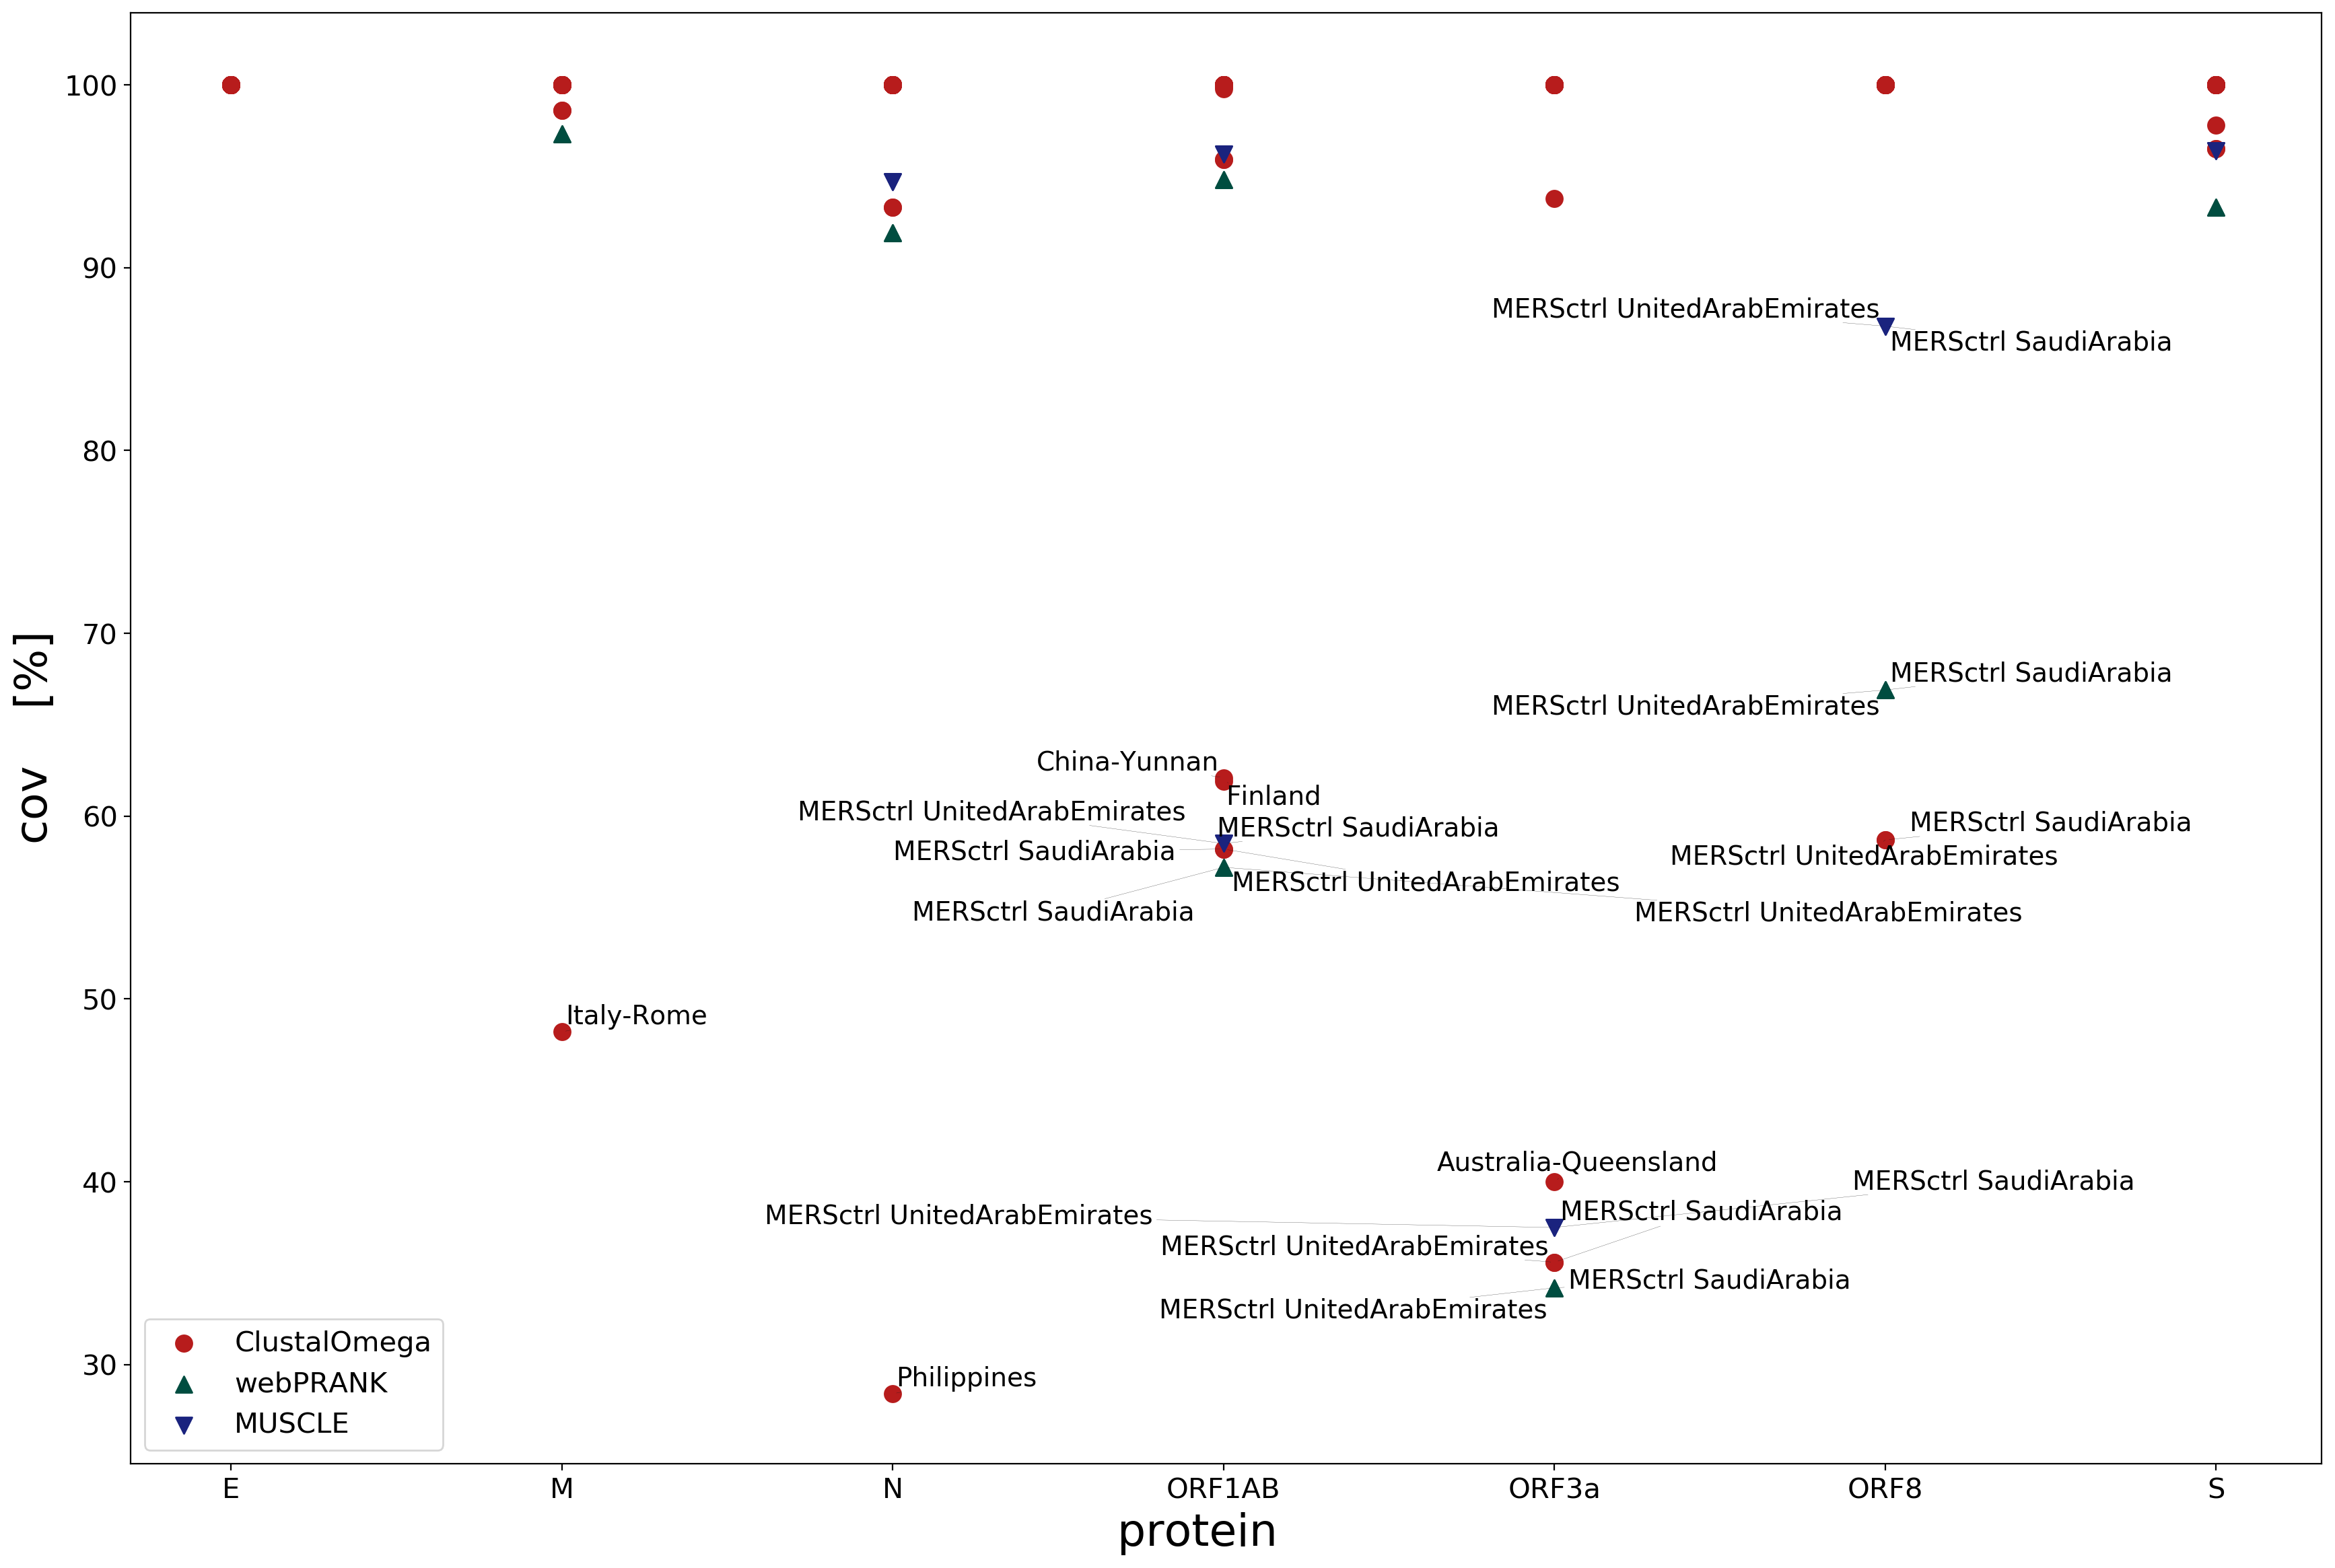
\includegraphics{images/05631a02-fe31-456c-a8ef-417a8b0abdda-uplt_protein_vs_cov.png}}{}
\makeatother 
\caption{{$cov $ values calculated with MView for all sequences of each protein sequence, using China's Dec2019 sequence as reference with Equation~(\ref{dfg-11ef4497176d}).}}
\label{f-c08c4047352a}
\end{figure*}
\egroup
As detailed in Figure~\ref{f-c08c4047352a}, the MERS sequences have a low percentage coverage in relation to the SARS-CoV-2 sequences with in about$60\% $ values. Some other SARS-CoV-2 sequences share low percentage values with the MERS sequences, following are some explanations:



\begin{itemize}
  \item \relax The EBI's database stores a short sequence of M\_Italy-Rome\_Jan2020, for that reason the alignment added a sequence of gaps in order to match the alignment. M\_Italy-Rome\_Jan2020 covers a small fragment of the hole sequence, hence the small coverage value. Similar cases apply for N\_Philippines\_2020Jan23, N\_Philippines\_2020Jan26, N\_Philippines\_2020Feb06, and ORF3a\_Australia-Queensland\_Feb2020
  \item \relax ORF1a\_Finland\_29Jan2020, and ORF1a\_China-Yunnan\_17Jan2020 were expected to have a low coverage as the reference sequence assess protein ORF1ab (not ORF1a). They were added to confirm the difference and discard a possible typo mistake.
\end{itemize}
  In summary, the $cov $ parameter describes how many 'gaps' are added to the alignment to achieve a better fit.


\bgroup
\fixFloatSize{images/90f1d9b1-53d0-4b96-bd86-e4490c95bb44-uplt_protein_vs_pid.png}
\begin{figure*}[!htbp]
\centering \makeatletter\IfFileExists{images/90f1d9b1-53d0-4b96-bd86-e4490c95bb44-uplt_protein_vs_pid.png}{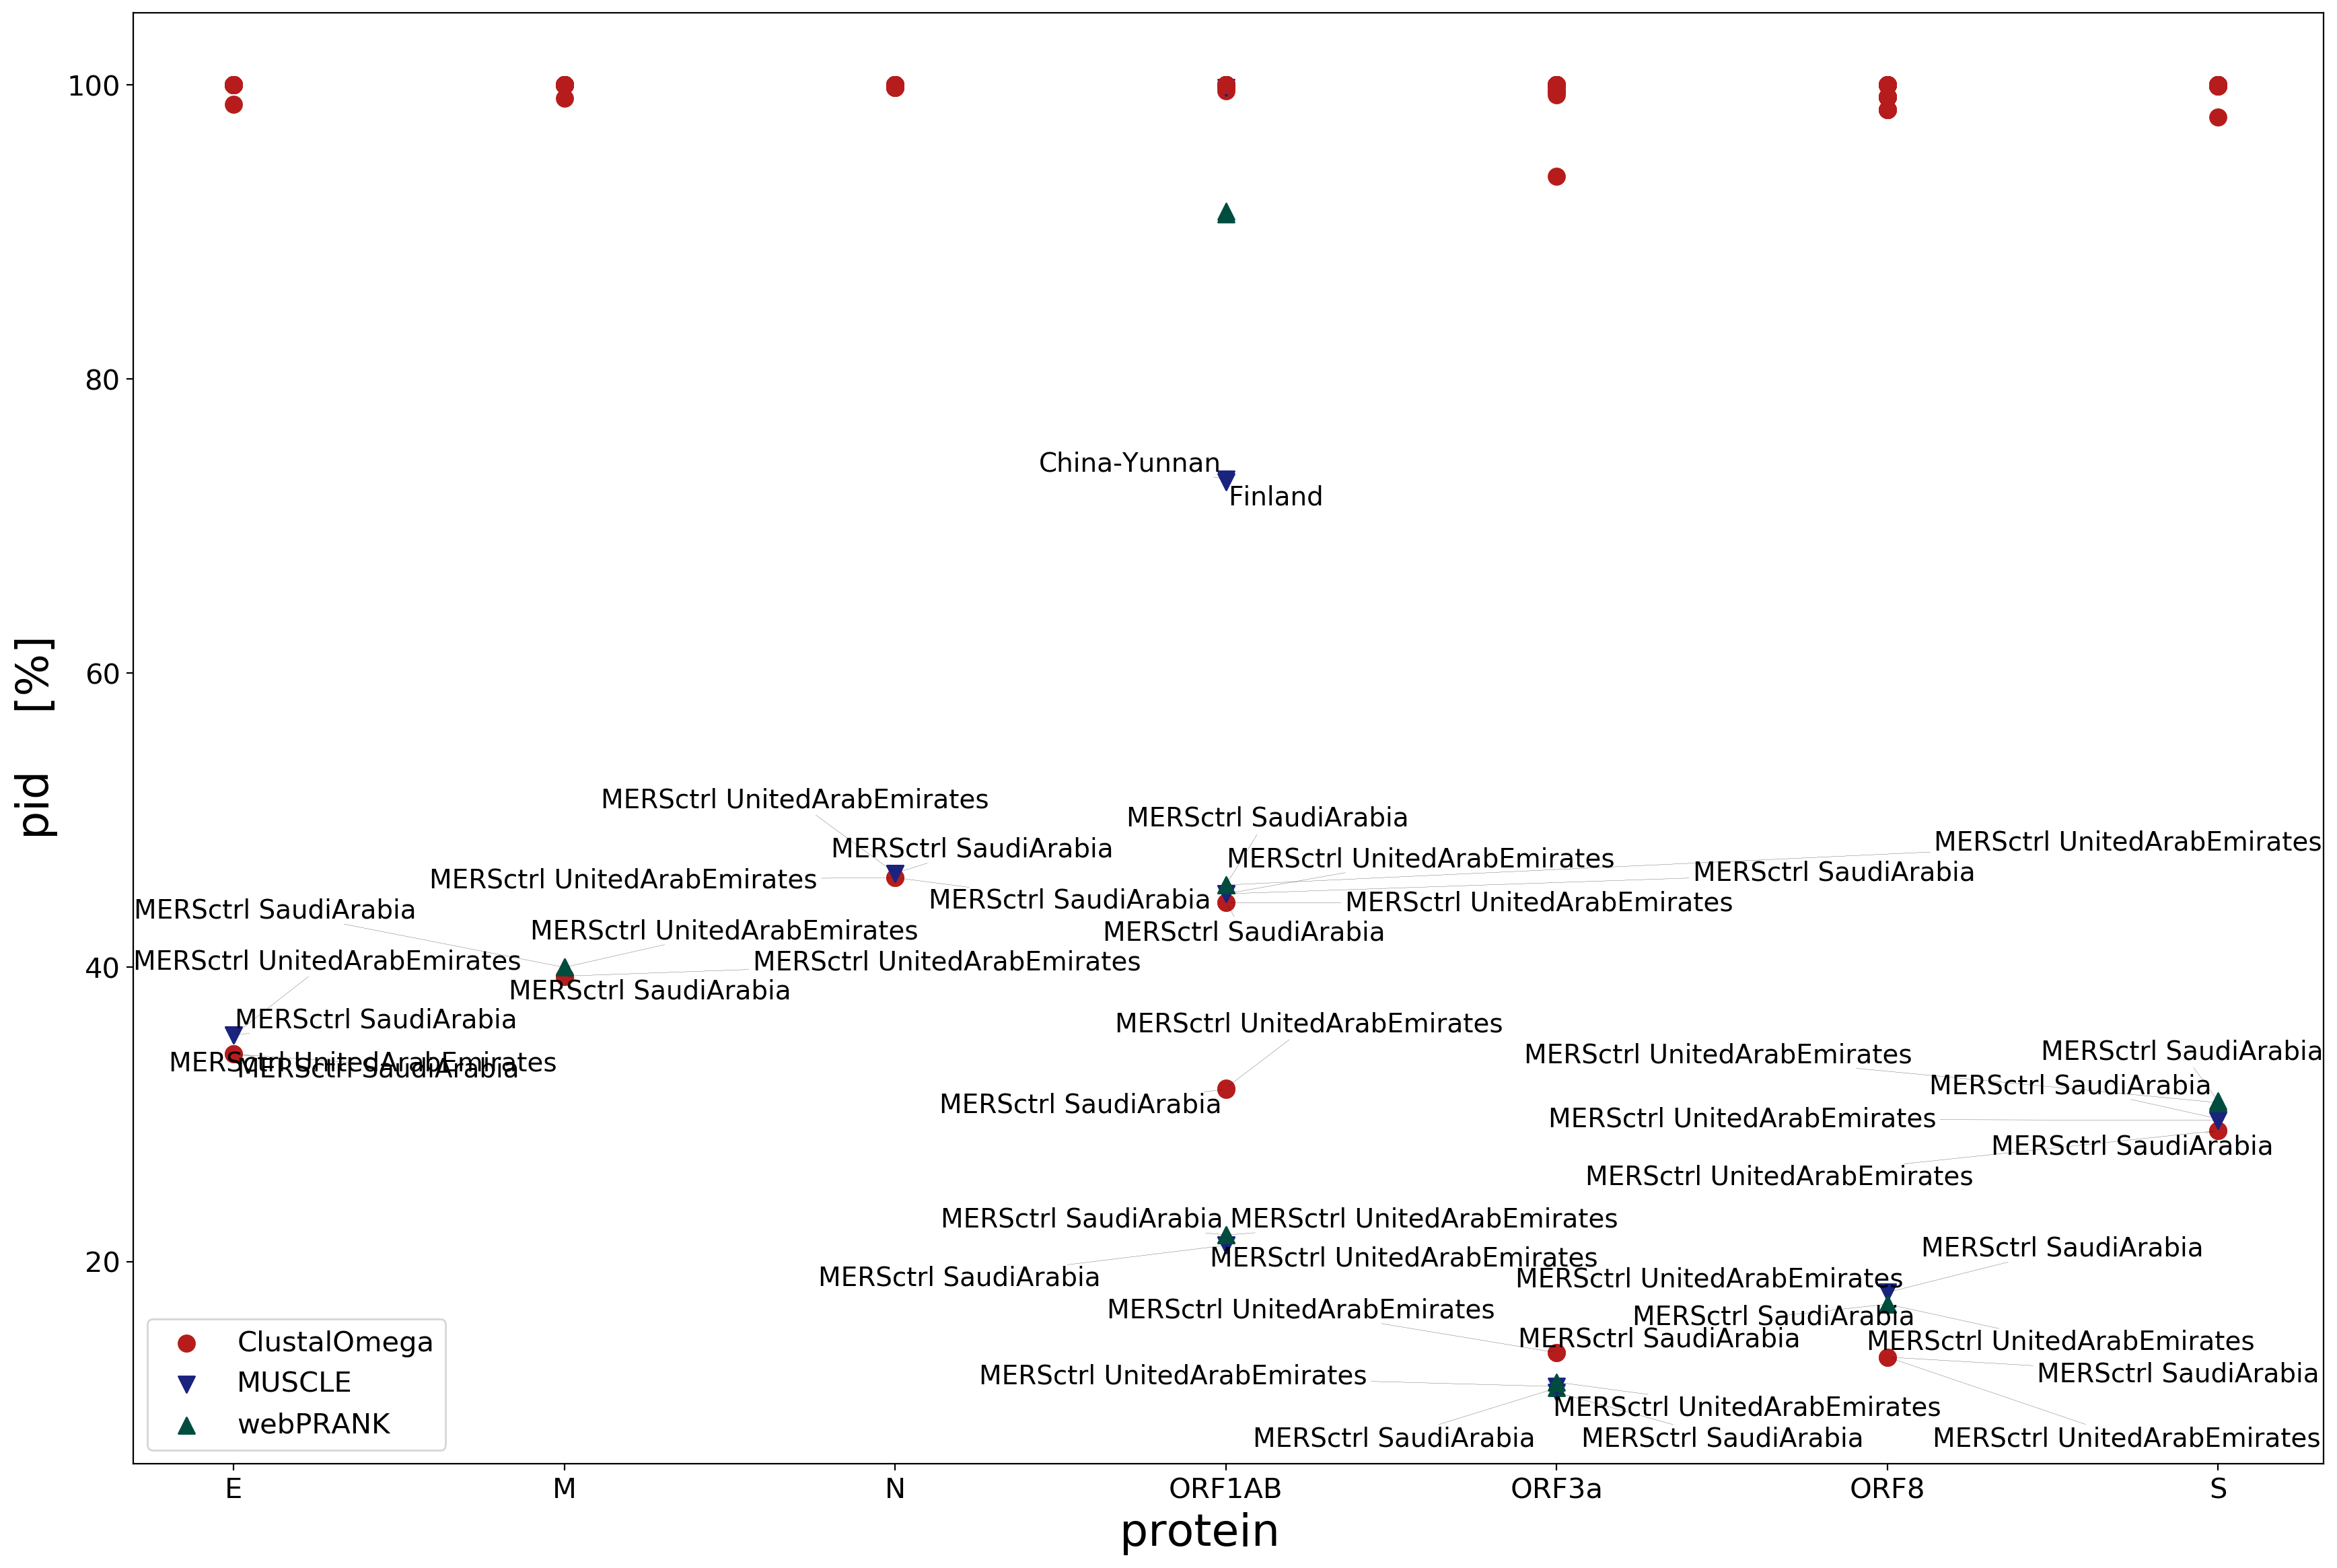
\includegraphics{images/90f1d9b1-53d0-4b96-bd86-e4490c95bb44-uplt_protein_vs_pid.png}}{}
\makeatother 
\caption{{$pid $ values calculated with MView for all sequences of each protein sequence, using China's Dec2019 sequence as reference with Equation~(\ref{dfg-3d2f6351284e}).}}
\label{f-216a5e4c828e}
\end{figure*}
\egroup
Figure~\ref{f-216a5e4c828e} plots the $pid $ calculations. As expected, only the MERS sequences have low identification values (confirming that they are different from the SARS-CoV-2). ORF1a\_Finland\_29Jan2020, and ORF1a\_China-Yunnan\_17Jan2020 also share a low $pid $, further explaining Figure~\ref{f-c08c4047352a}'s conclusion.

\clearpage 
    

\bibliographystyle{blank}

\bibliography{\jobname}

\section*{Author biography}

\bioItem[images/bf0f1284-fa36-4678-a9e7-05671376e50c-umeitesm]{Antonio Osamu Katagiri Tanaka}{ .

MNT16

A01212611}
\printBio 

\end{document}
